\documentclass[10pt]{beamer}

\usepackage[utf8]{inputenc}
\usepackage[english, russian]{babel}
\usepackage{hyperref}
\usepackage{enumerate}
\usepackage{amsmath}
\usepackage{graphicx}
\usepackage{mathtools}
\usepackage{tikz}
\usepackage{xcolor}
\hypersetup{
    colorlinks,
    linkcolor=black,
    urlcolor={blue!80!black}
}
\usetikzlibrary{positioning}
\linespread{1.5}

\newcommand{\E}{\mathrm{E}}
\newcommand{\hy}{\mu(X^l)}
\newcommand{\Exy}{\E_{x,y}}
\newcommand{\El}{\E_{X^l}}
\newcommand{\p}{\partial}
\newcommand{\Sum}{\sum\limits}
\renewcommand\i{\textit}
\renewcommand\thesection{}
\newcommand\und\textunderscore

\usetheme{Darmstadt}

\begin{document}

\title{Гладкие метрики в задаче ранжирования}
\author[]
{
\begin{tabular}{rl}
Научрук: & \href{https://staff.yandex-team.ru/graf-vk}{Александр Воронцов} \\
Студент: & \href{https://staff.yandex-team.ru/mlevkov}{Мирон Левков}
\end{tabular}
}

\frame{\titlepage}
\date{}

\begin{frame}
\frametitle{Проблема}

У метрик ранжирования есть одна проблема - метрика меняется лишь при перестановке двух документов местами. 
Таким образом метрики не имеют гладкой зависимости от скоров, выдаваемых ранжирующим алгоритмом.
\end{frame}


\begin{frame}
\frametitle{Постановка задачи}

$$\boxed {DCG = \Sum_{i=1}^p \frac{rel_i}{discount(i)}}$$

Целью работы является поиск метрики ранжирования, которая удовлетворяет следующим свойствам:
\begin{itemize}
\item Данная метрика является является достаточно гладкой (о том, как измерялась гладкость, далее)
\item Данная метрика достаточно хорошо линейно аппроксимирует DCG, т.е. $DCG \simeq \alpha \cdot metric + \beta$
\end{itemize}
\end{frame}


\begin{frame}
\frametitle{Применение результатов}
Гладкий аналог метрики DCG является более чувствительным способом измерения качества модели.
\begin{itemize}
\item Смешивание моделей
\item Отбор признаков
\item Кривая обучения модели
\item Добавление шума в качестве sanity-check
\end{itemize}
\end{frame}


\begin{frame}
\frametitle{Метрики качества результатов}
\begin{enumerate}
\item Гладкость кривой (значения метрики с изменением некоего параметра - например, коэффициента смеси двух формул)
определялась так:
$$\frac{1}{n - window} \Sum_{i=1}^{n - window} (poly_{deg}(y_i,\dots,y_{i + window - 1})_{i + \frac{window}{2}} - y_{i + \frac{window}{2}})^2$$
\item Аппроксимация метрики DCG считалась, так:\\
$$\underset{\alpha, \beta}{\min} ~ MSE(values_{dcg}, \alpha \cdot values_{metric} + \beta)$$
\end{enumerate}
\end{frame}


\begin{frame}
\frametitle{Рассмотренные метрики. SoftDCG}
\begin{enumerate}
\item Сопоставим каждому документу нормальное распределения с некими параметрами.
\item Посчитаем мат ожидание позиции в выдаче для каждого документа, чтоб использовать 
средний discount \cite{SoftDCGPaper}
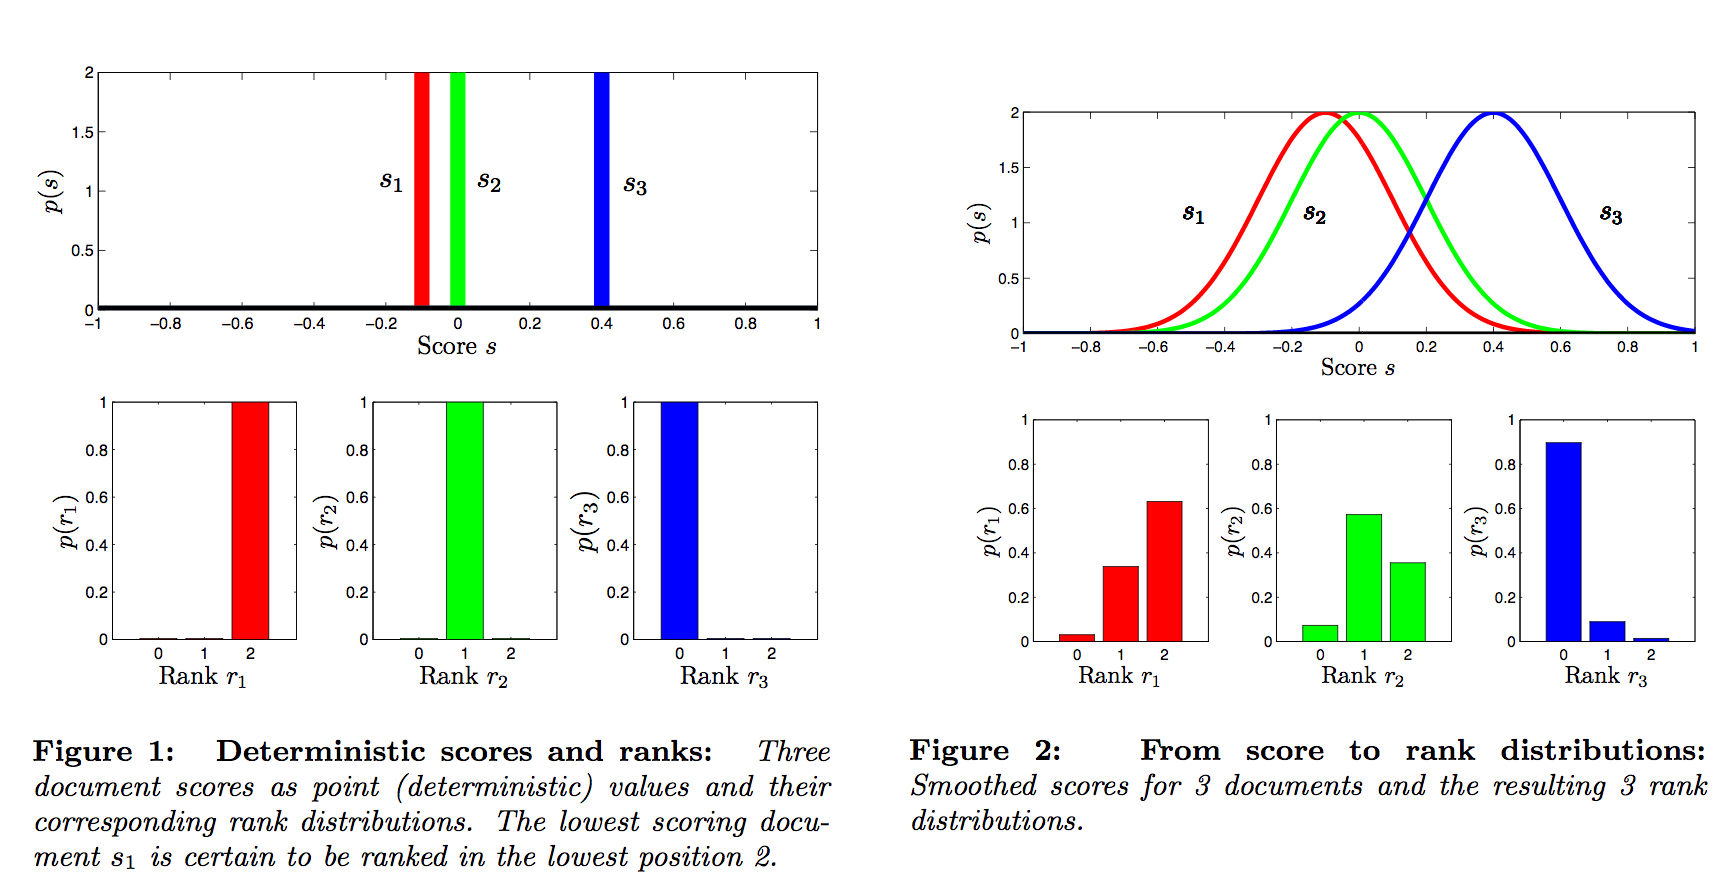
\includegraphics[width=3.5in]{SoftDCG}
\end{enumerate}
\end{frame}


\begin{frame}
\frametitle{Рассмотренные метрики. NoisedSoftDCG}
\begin{enumerate}
\item Сгенерируем случайный шум и добавим его к скорам
\item Посчитаем средний DCG по m зашумлениям
\item Шум может менять между собой близкие по скорам документы тем самым 
сглаживая метрику при усреднении
\end{enumerate}
\end{frame}


\begin{frame}
\frametitle{Рассмотренные метрики. FairSoftDCG}
\begin{enumerate}
\item Будем интерпретировать скоры, как вероятности документов находиться на своих позициях.
Т.е. $P(doc_i > doc_j) = \frac{e^{\sigma s_i}}{e^{\sigma s_i} + e^{\sigma s_j}}$
\item Можно ввести распределение на всех перестановках документов 
\item Посчитаем мат ожидание DCG по всем перестановкам документов в top-k
\end{enumerate}
\end{frame}


\begin{frame}
\frametitle{Гладкость метрик при изменении размера пула}
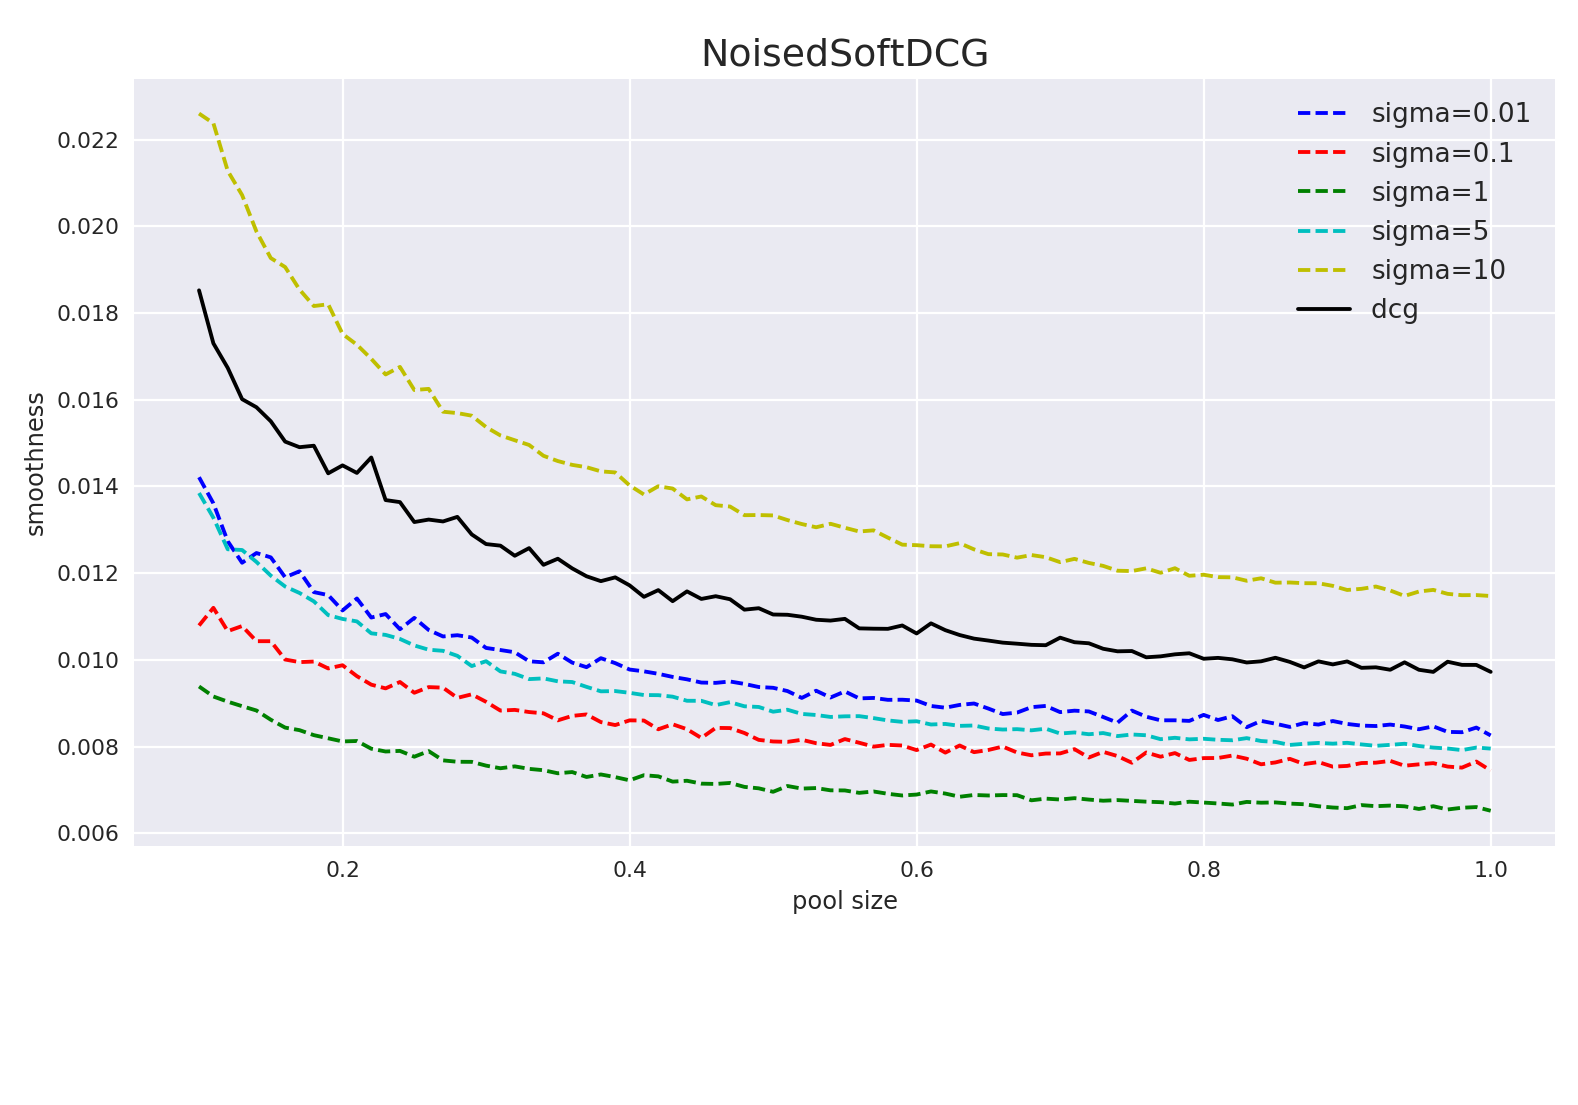
\includegraphics[width=\textwidth]{noised_decrease_smoothness}
\end{frame}


\begin{frame}
\frametitle{Гладкость метрик при изменении размера пула}
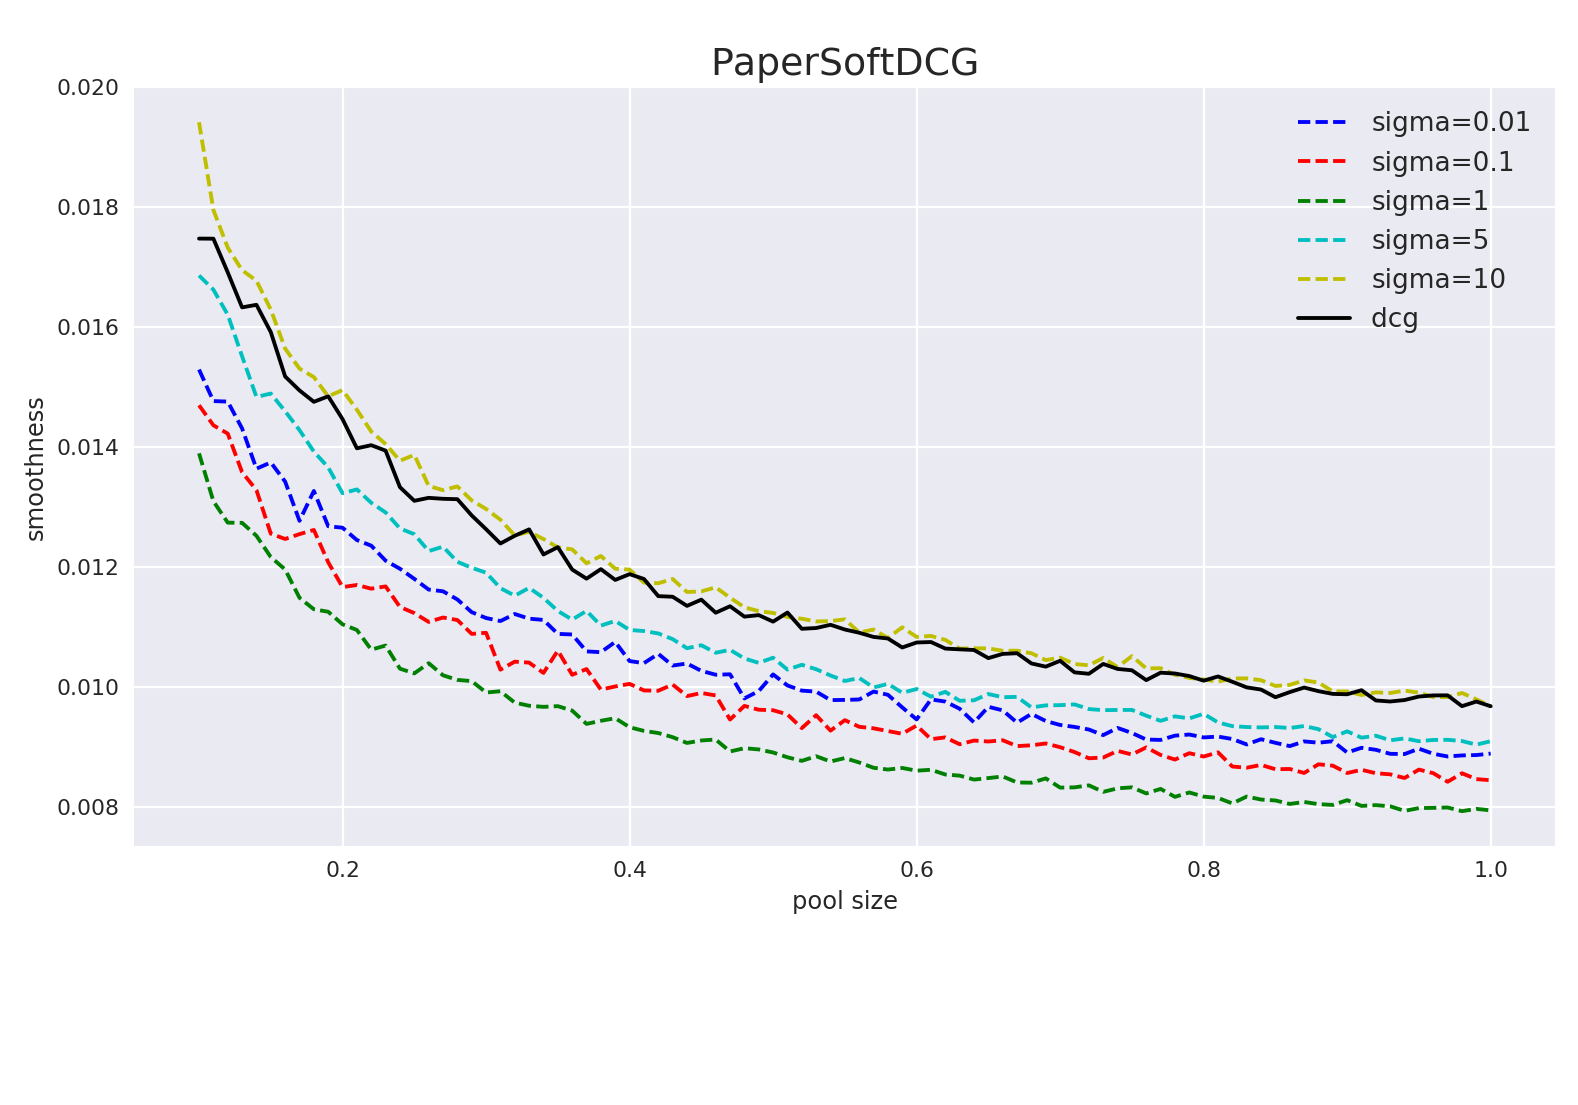
\includegraphics[width=\textwidth]{paper_decrease_smoothness}
\end{frame}


\begin{frame}
\frametitle{Аппроксимация DCG при изменении размера пула}
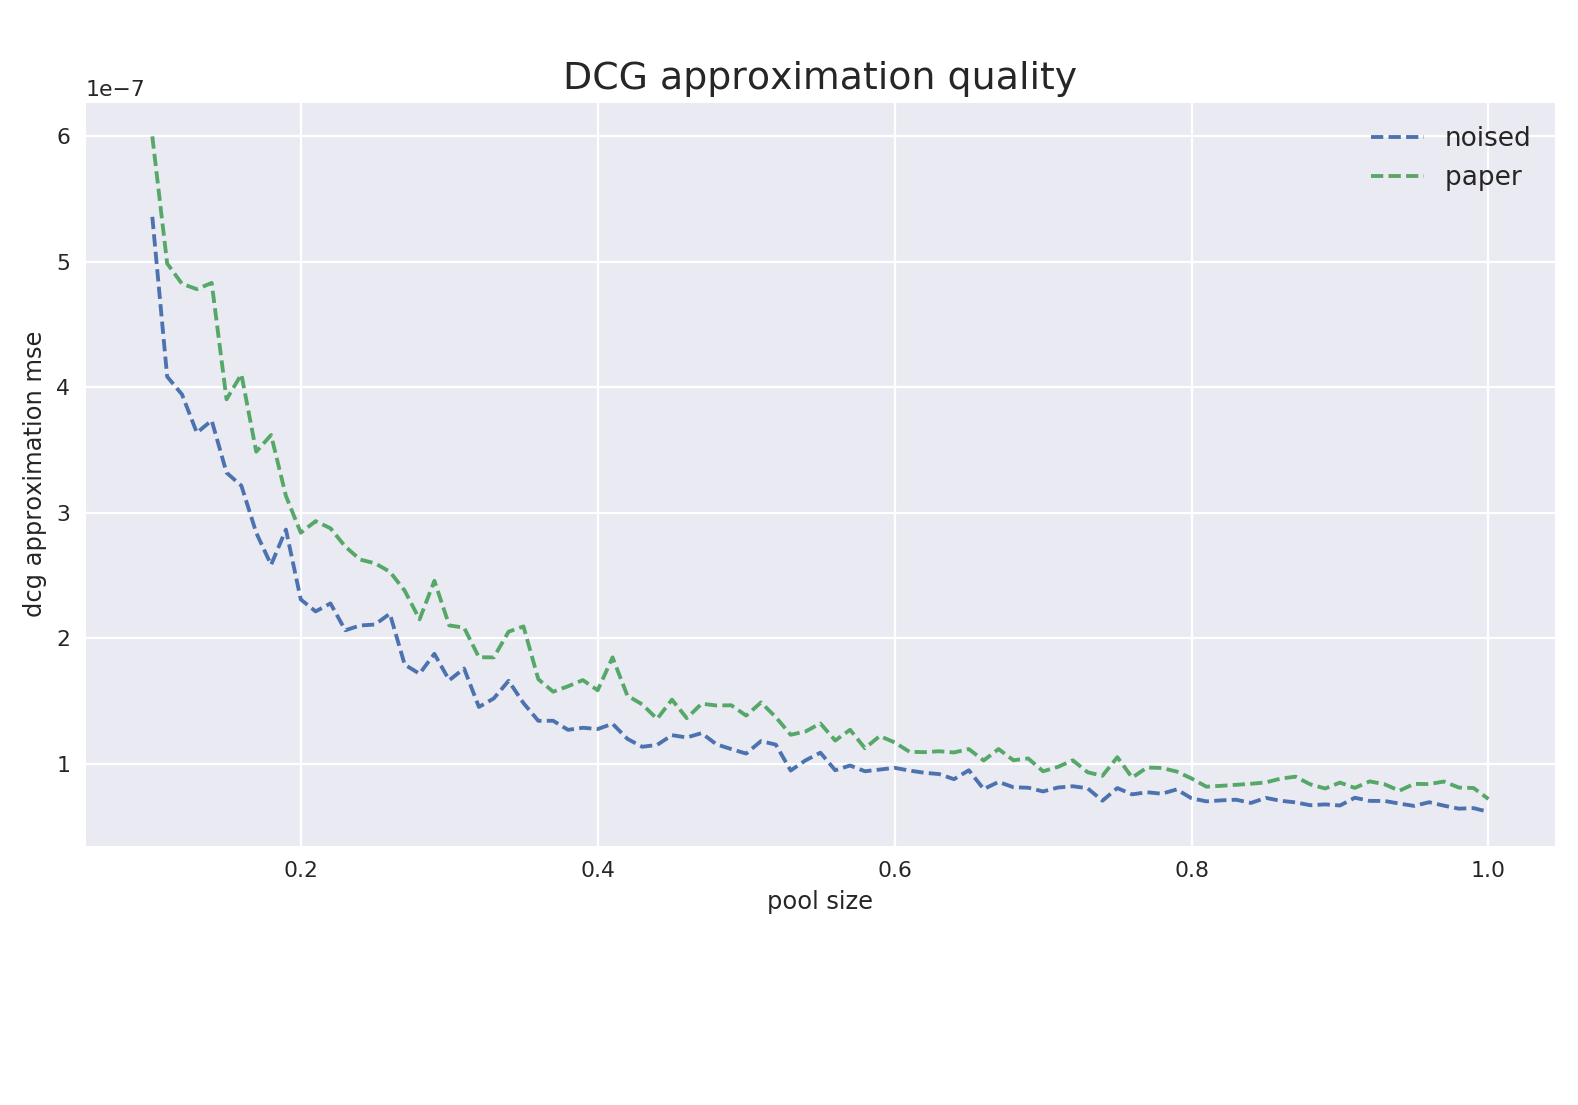
\includegraphics[width=\textwidth]{dcg_approximation}
\end{frame}


\begin{frame}
\frametitle{Изменение метрик при зашумлении}
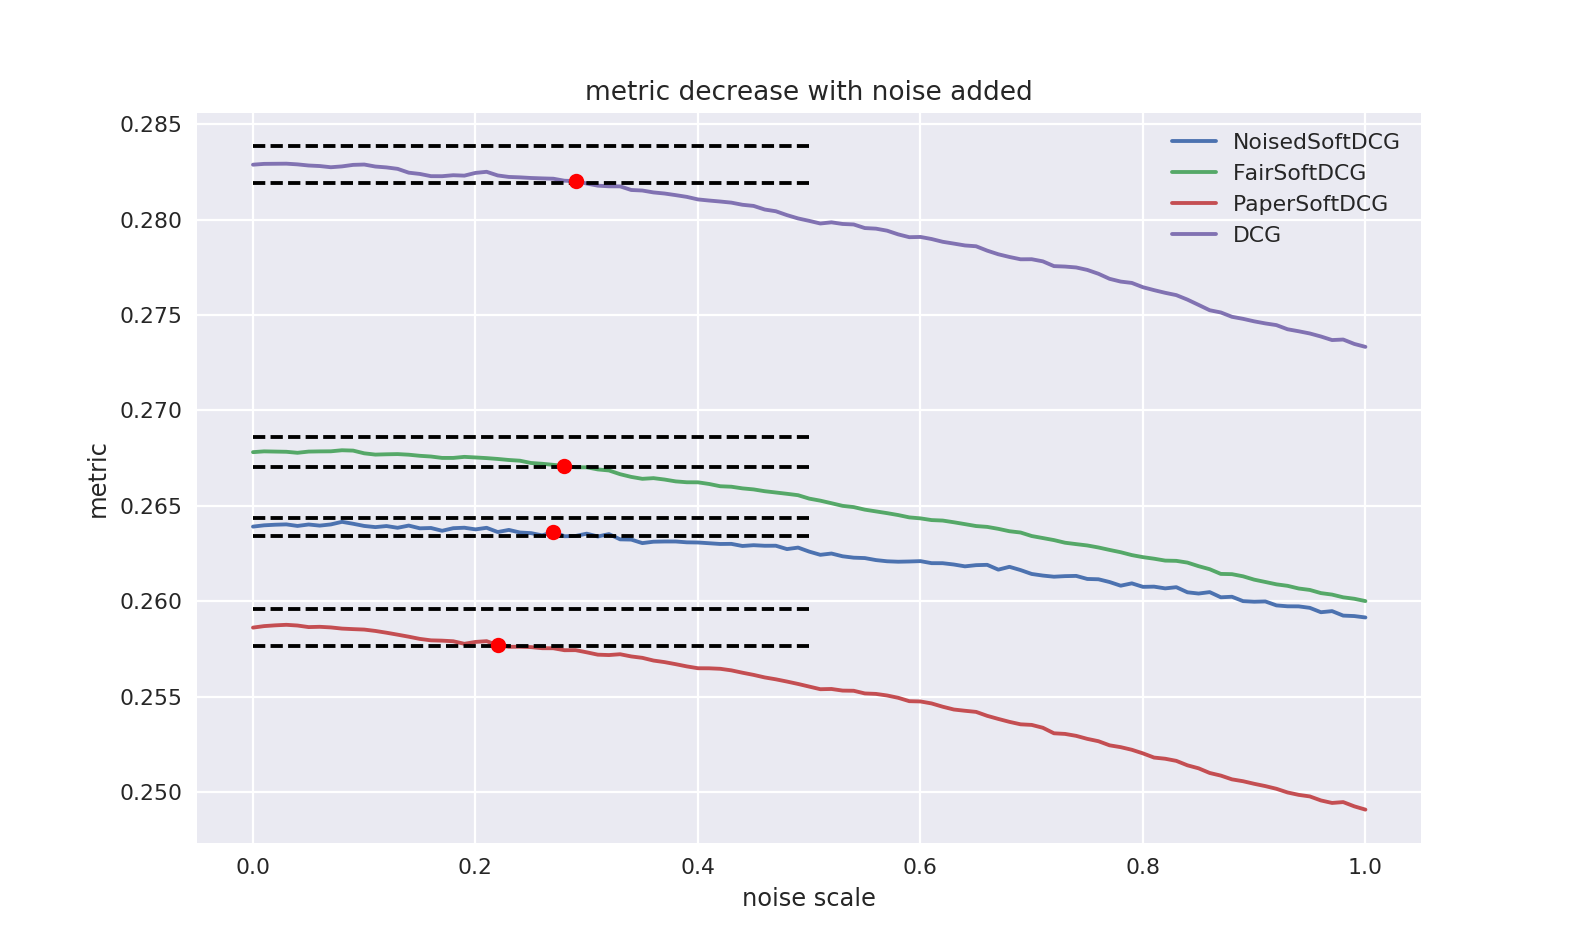
\includegraphics[width=\textwidth]{noised_metrics}
\end{frame}


\begin{frame}
\frametitle{Метрика для выпуклой комбинации формул (max/min)}
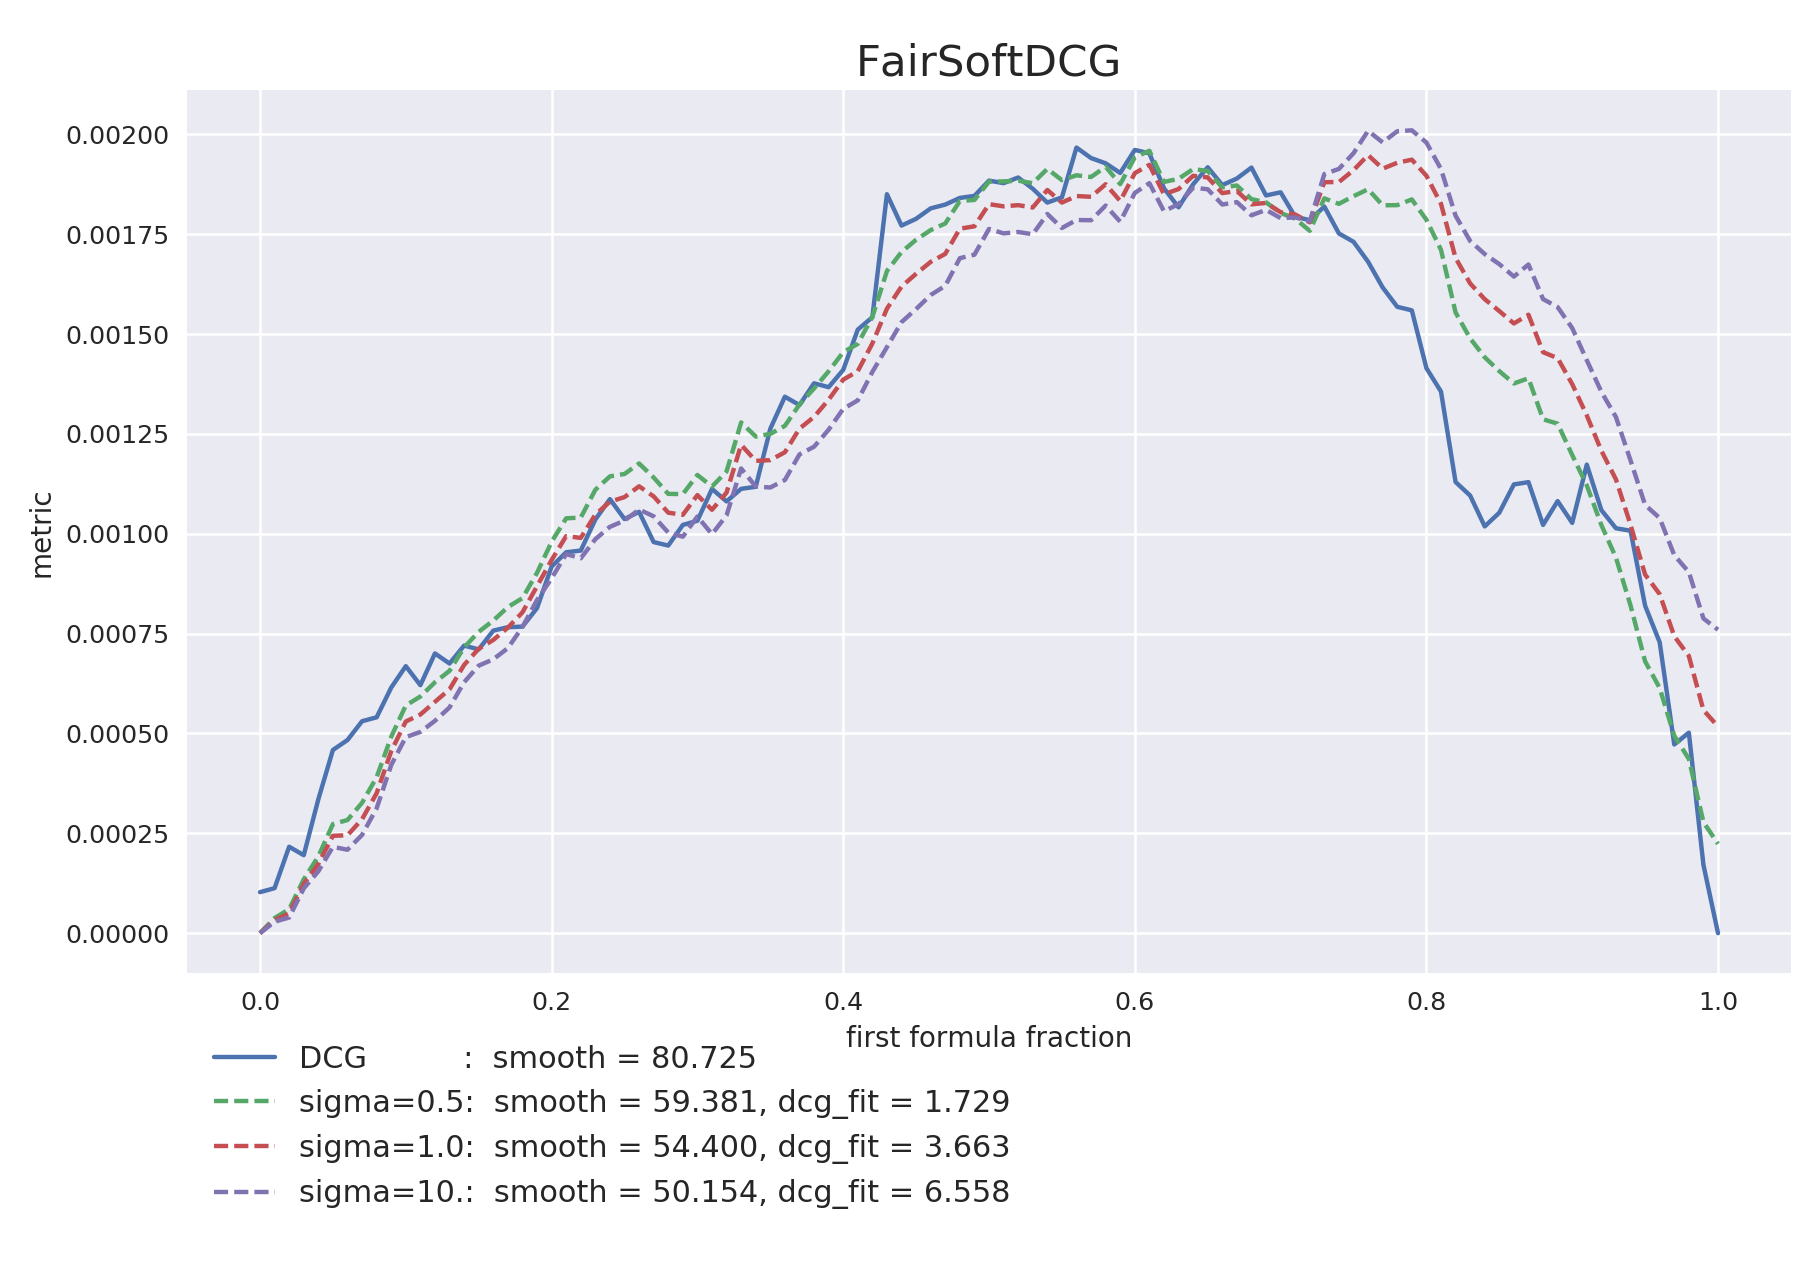
\includegraphics[width=\textwidth]{fair_formula_mix}
\end{frame}


\begin{frame}
\frametitle{Метрика для выпуклой комбинации формул (max/min)}
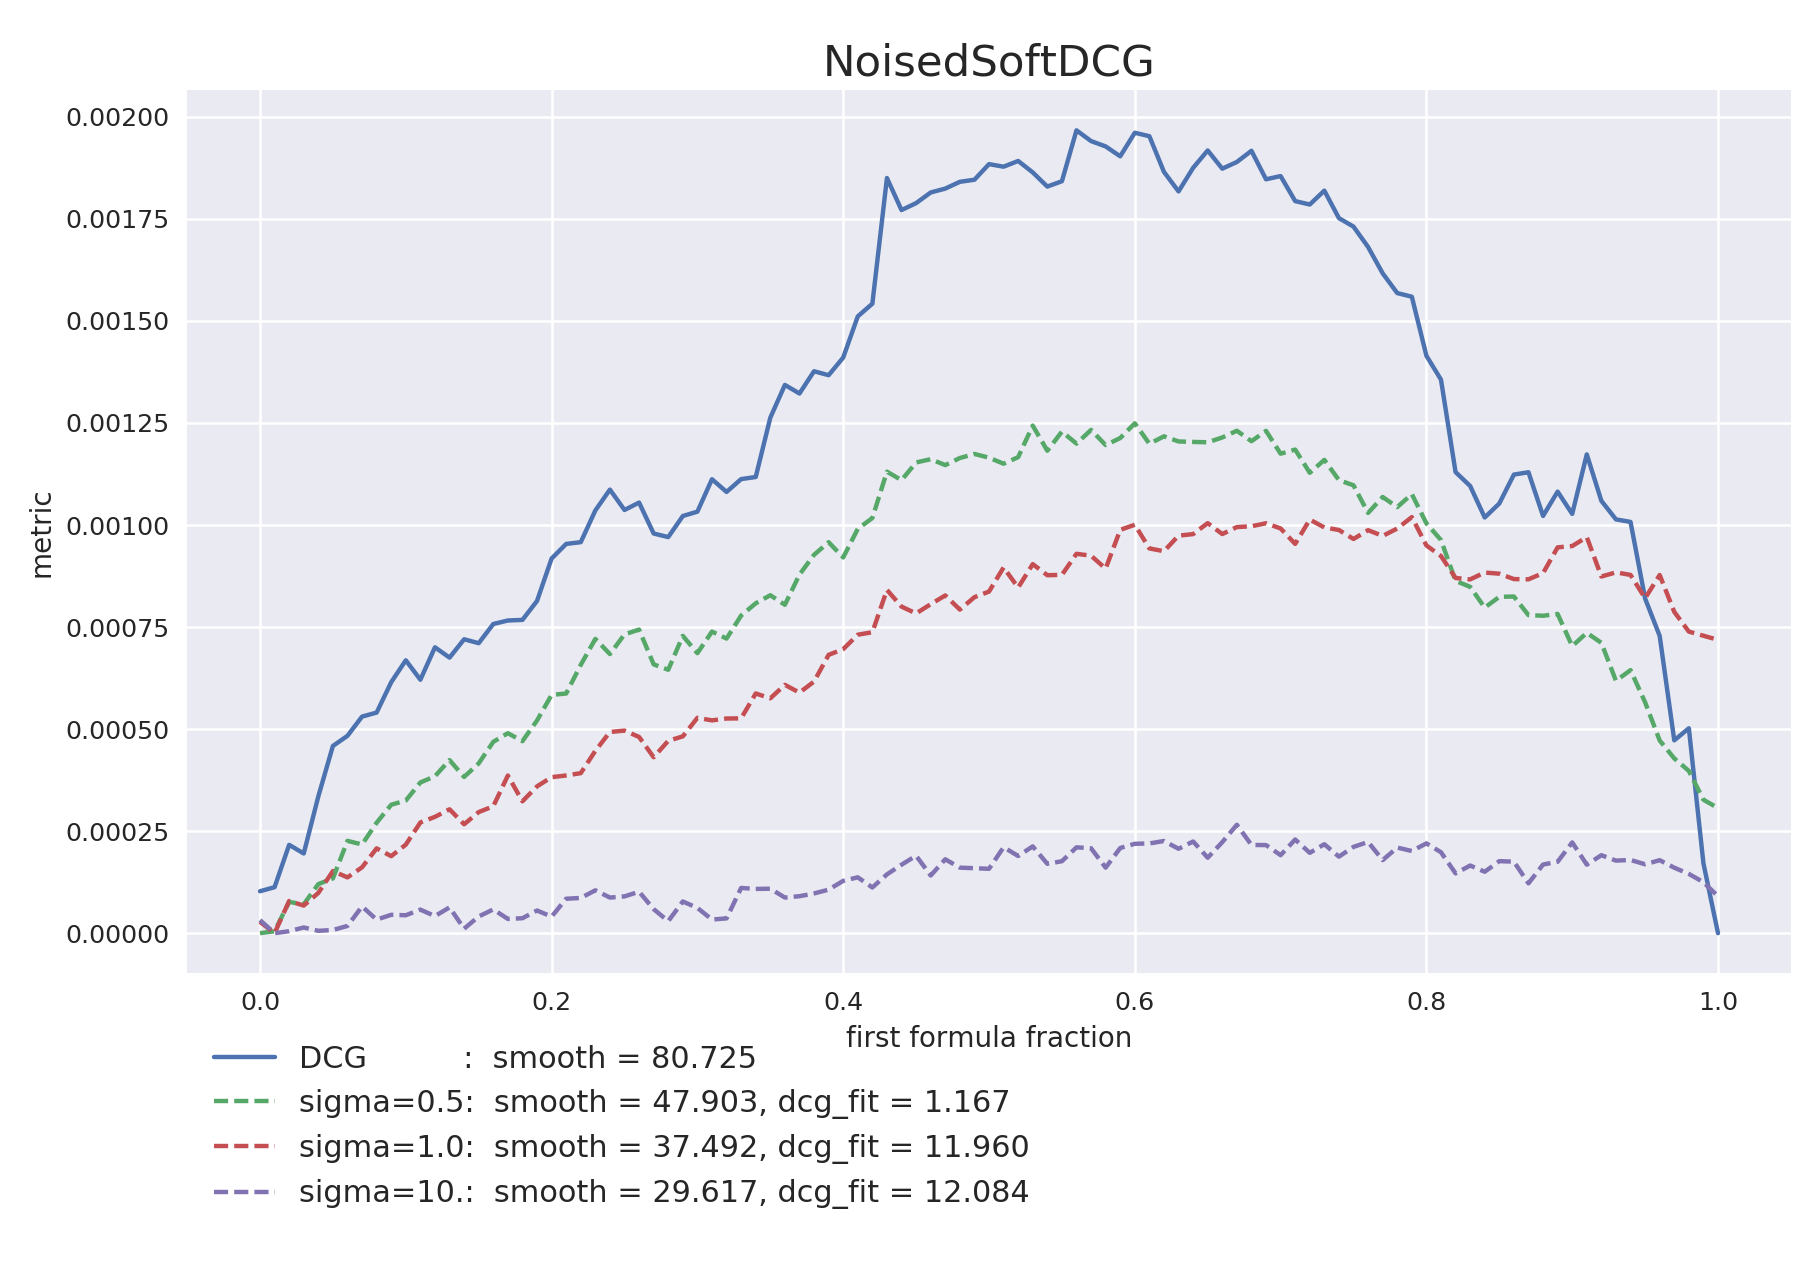
\includegraphics[width=\textwidth]{noised_formula_mix}
\end{frame}


\begin{frame}
\frametitle{Метрика для выпуклой комбинации формул (max/min)}
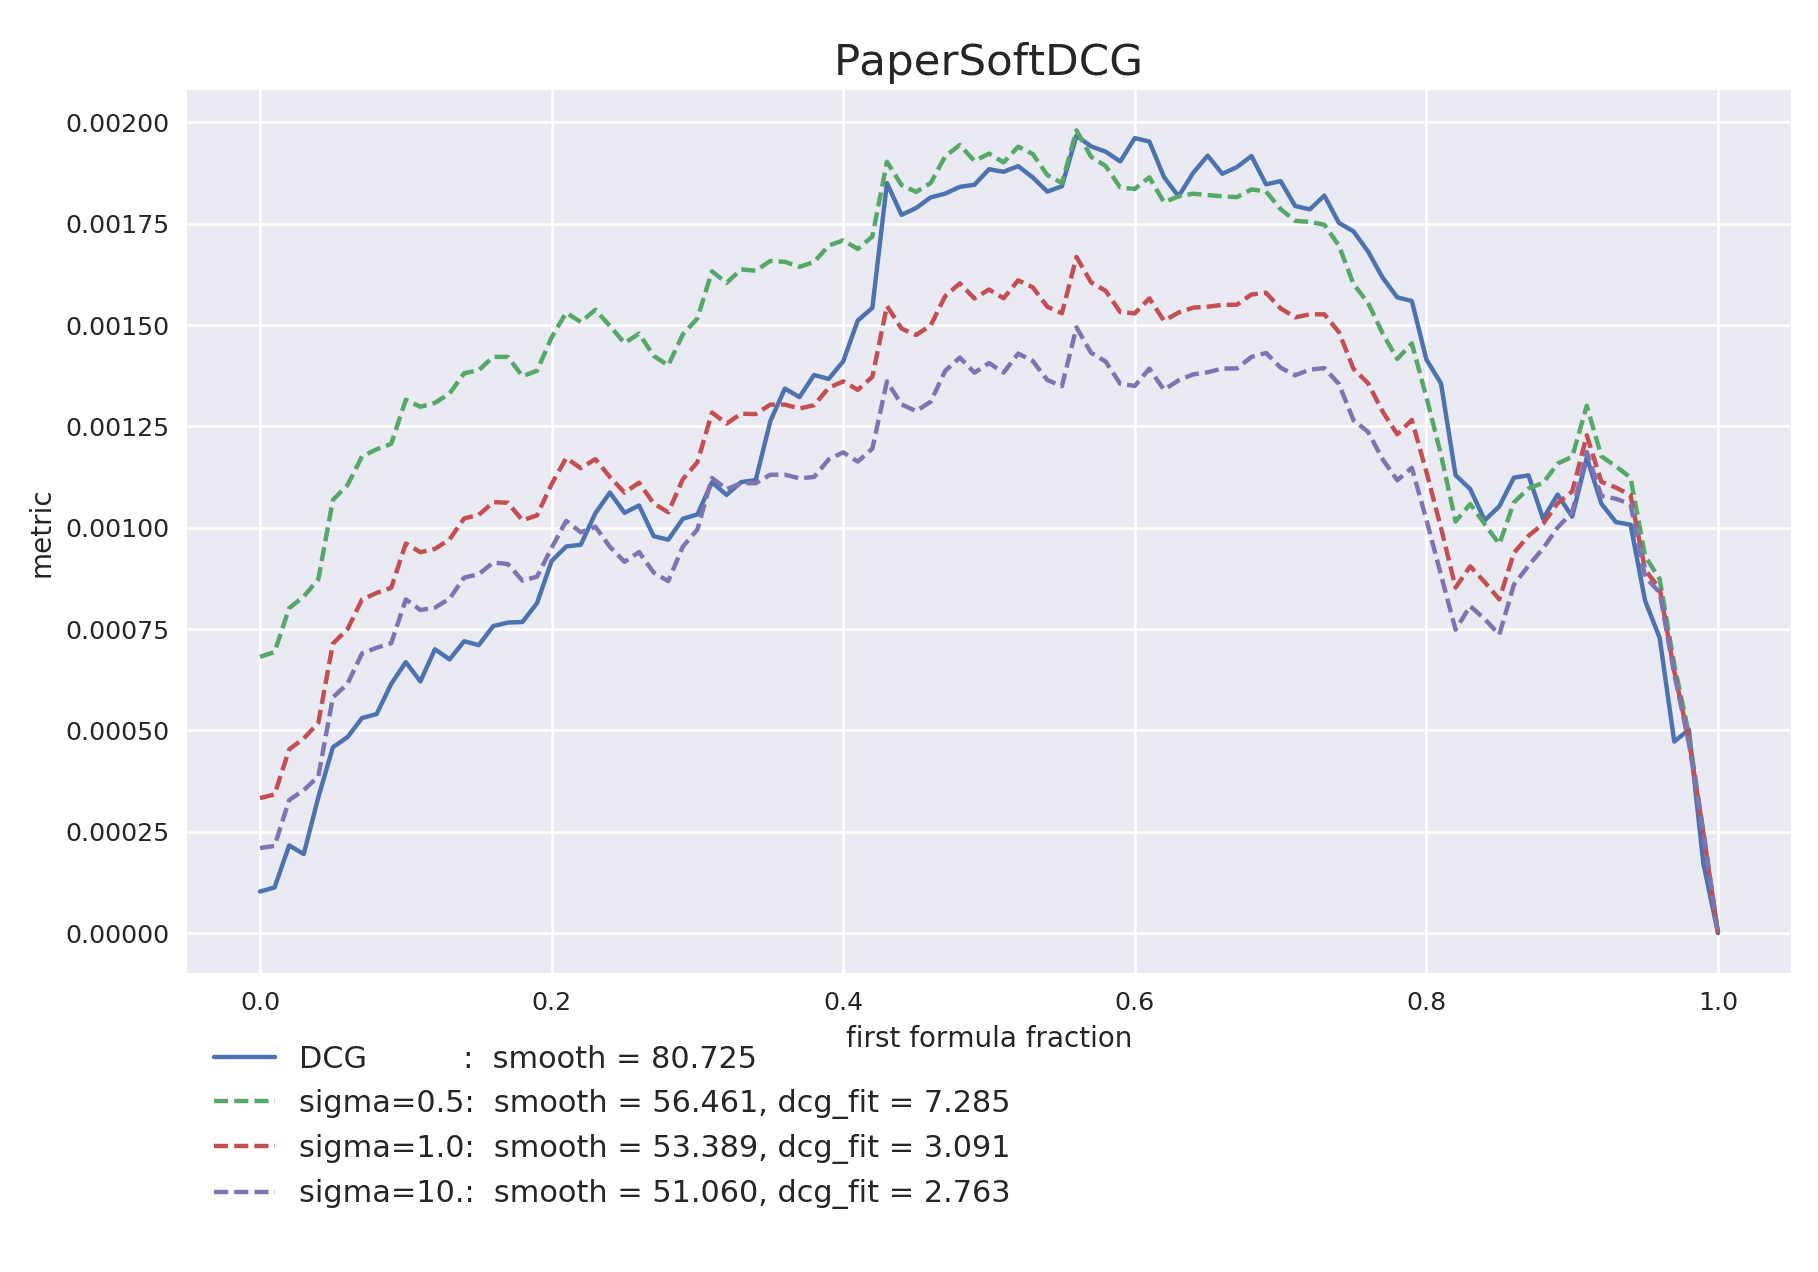
\includegraphics[width=\textwidth]{paper_formula_mix}
\end{frame}


\begin{frame}
\frametitle{Метрика для выпуклой комбинации формул (std)}
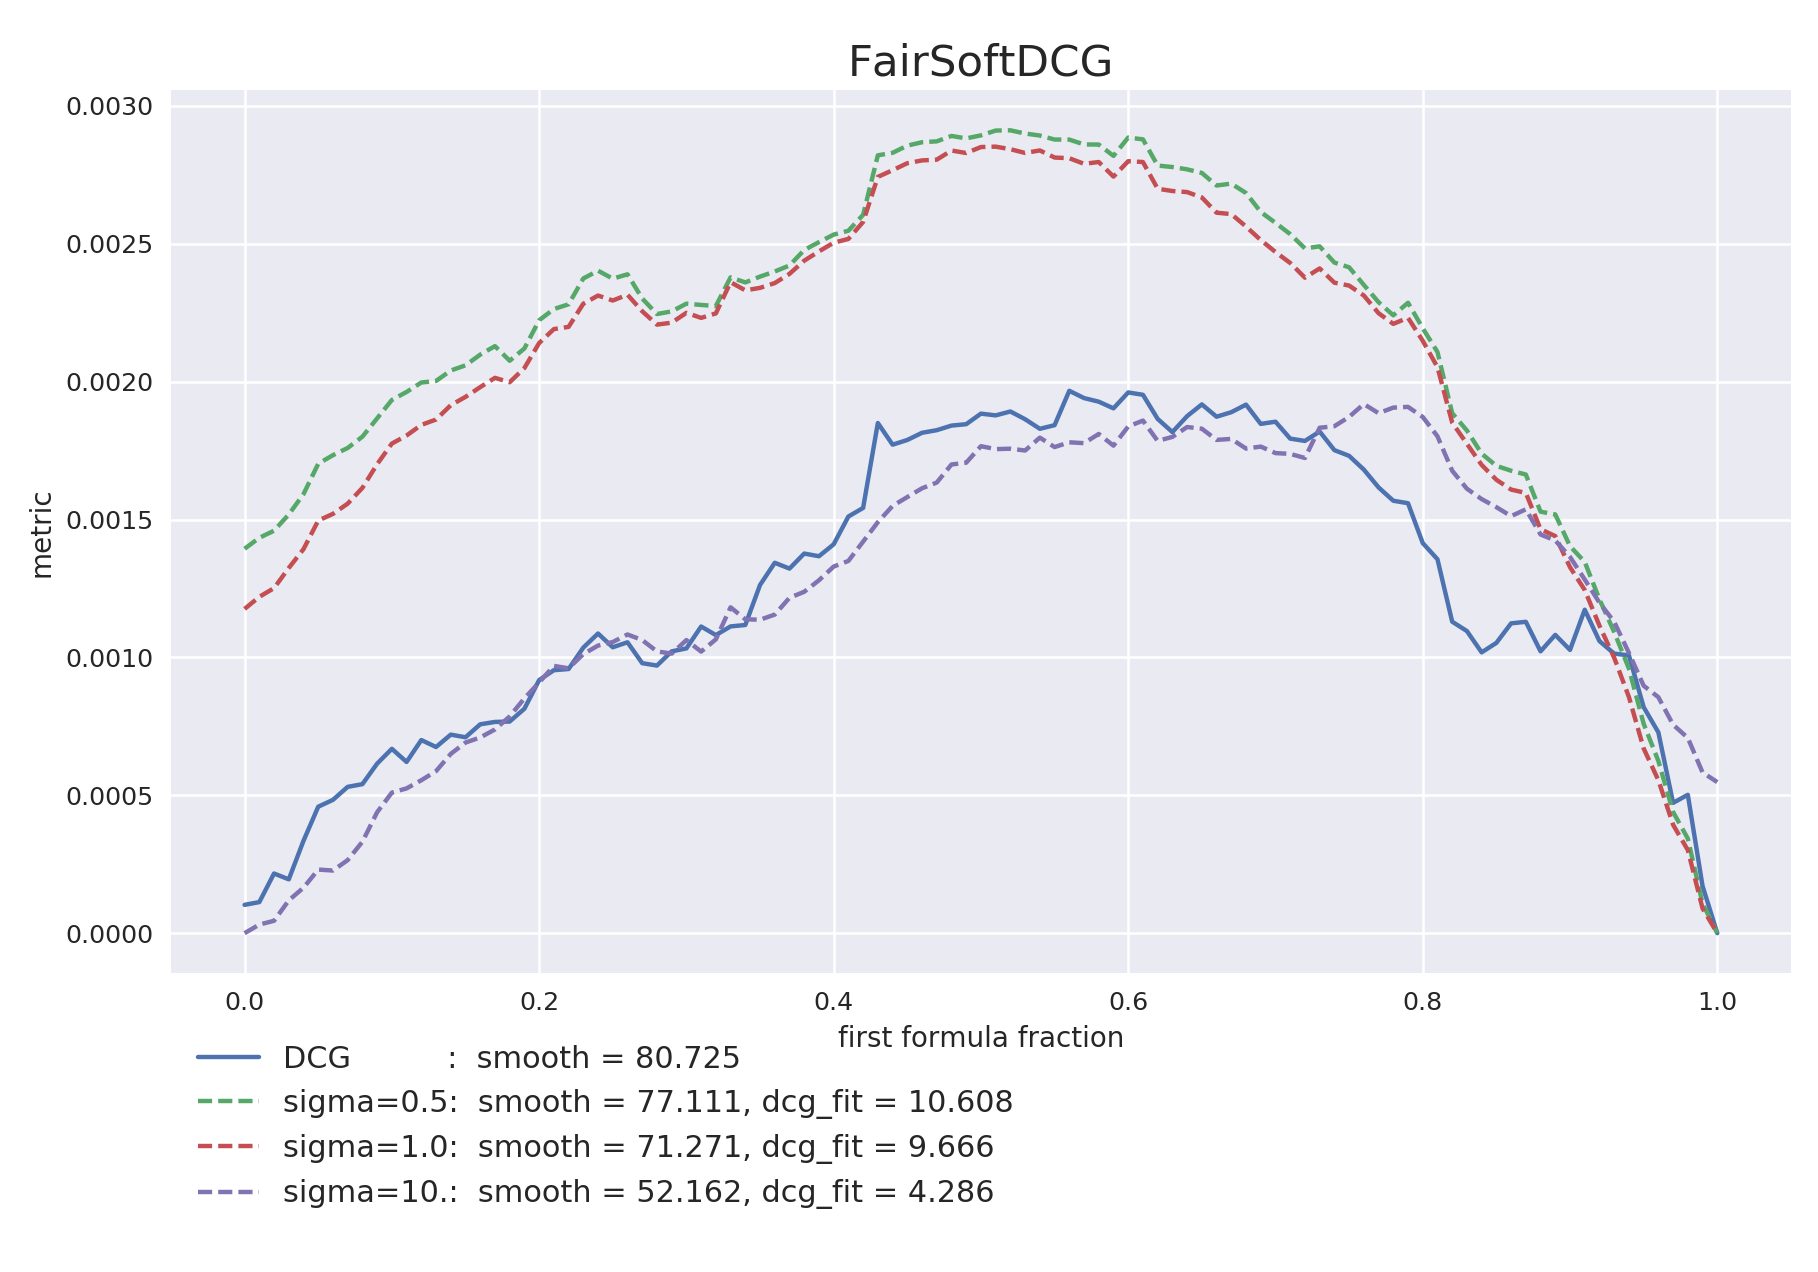
\includegraphics[width=\textwidth]{fair_formula_mix_std}
\end{frame}


\begin{frame}
\frametitle{Выбор сигмы}
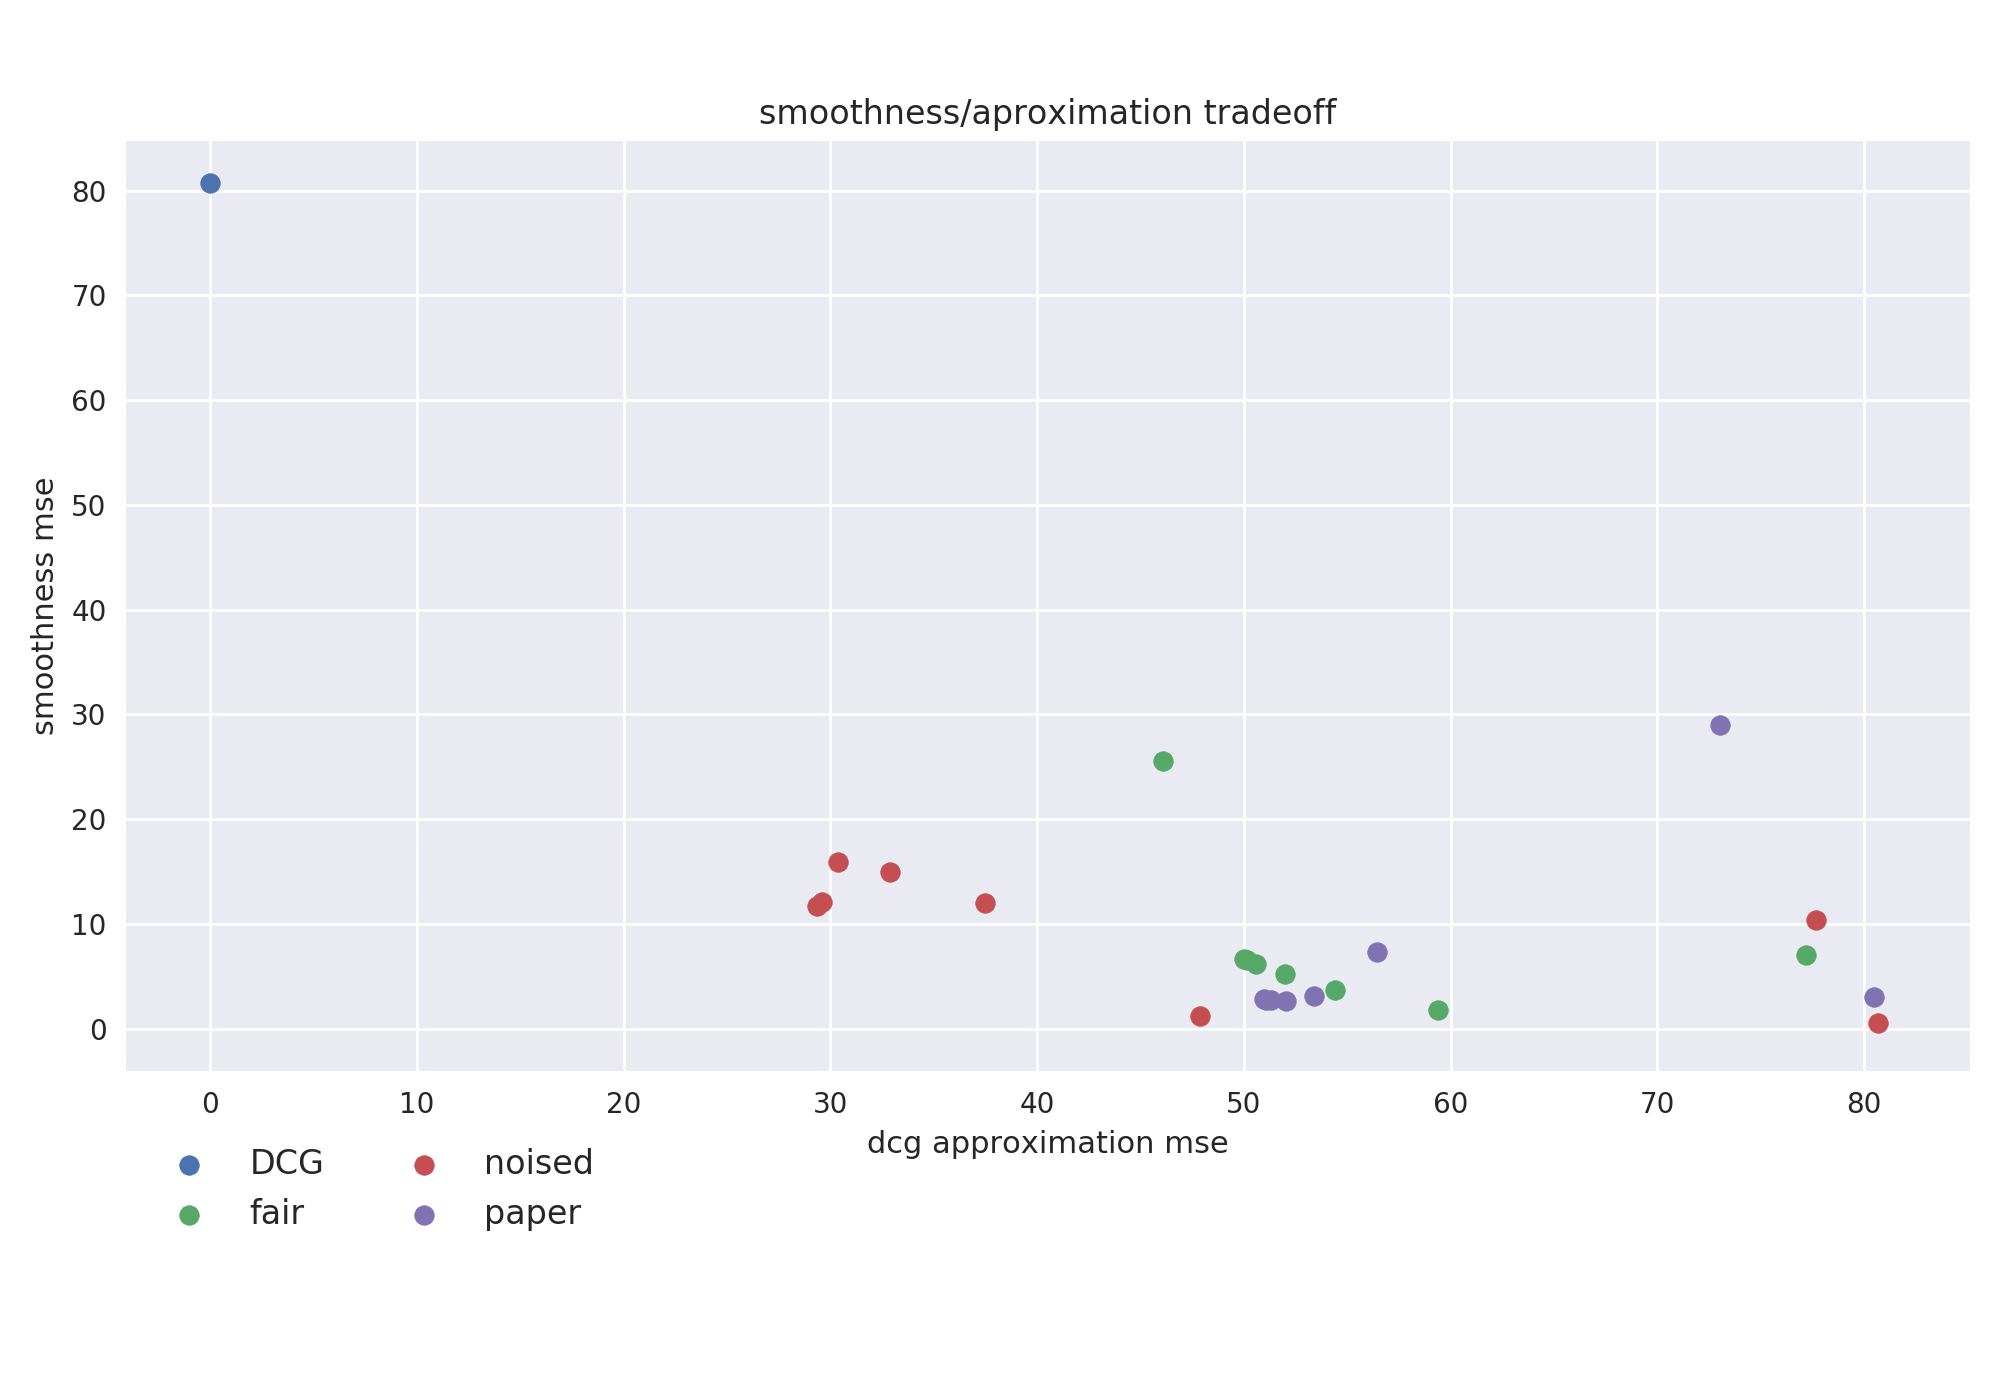
\includegraphics[width=\textwidth]{tradeoff_max_min}
\end{frame}


\begin{frame}
\frametitle{Проблемы}
\begin{enumerate}
\item Хочется выбирать параметр $\sigma$ нашей метрики автоматически
\item Наша метрика гладкости не является идеальной, т.к. тоже требует подбора параметров:
степень аппроксимирующего полинома, размер окна
\end{enumerate}
\end{frame}


\begin{frame}
\frametitle{Список литературы}
\begin{thebibliography}{1}
\setbeamertemplate{bibliography item}[text]

\bibitem{SoftDCGPaper} \href{https://www.microsoft.com/en-us/research/publication/softrank-optimising-non-smooth-rank-metrics/}
{M. Taylor, J. Guiver, S. Robertson and T. Minka. SoftRank: Optimising Non-Smooth Rank Metrics. Microsoft Research Cambridge, 2016}

\bibitem{LambdaMARTPaper} \href{https://www.microsoft.com/en-us/research/publication/from-ranknet-to-lambdarank-to-lambdamart-an-overview/}
{Christopher J.C. Burges. From RankNet to LambdaRank to LambdaMART. Microsoft Research Technical Report, 2010}

\bibitem{LearningToRankPaper} \href{https://www.microsoft.com/en-us/research/publication/learning-to-rank-from-pairwise-approach-to-listwise-approach/}
{Zhe Cao, Tao Qin, Tie-Yan Liu, Ming-Feng Tsai, Hang Li. Learning to Rank: From Pairwise Approach to Listwise Approach. Microsoft Research Technical Report, 2007}

\end{thebibliography}
\end{frame}



\begin{frame}
\begin{center}
\Huge Спасибо за внимание!
\end{center}
\end{frame}


\end{document}